\documentclass[tikz,border=8pt]{standalone}

\usepackage[T1]{fontenc}
\usepackage{xcolor}
\usetikzlibrary{arrows.meta,backgrounds,calc,fit,positioning}

\definecolor{rowblue}{HTML}{DCEAF7}
\definecolor{rowblueborder}{HTML}{3973A5}
\definecolor{colgreen}{HTML}{E2F0E7}
\definecolor{colgreenborder}{HTML}{3E7C59}
\definecolor{accentgold}{HTML}{C17D11}
\definecolor{repairred}{HTML}{A23B3B}
\definecolor{ink}{HTML}{20242A}
\definecolor{muted}{HTML}{606A76}

\begin{document}
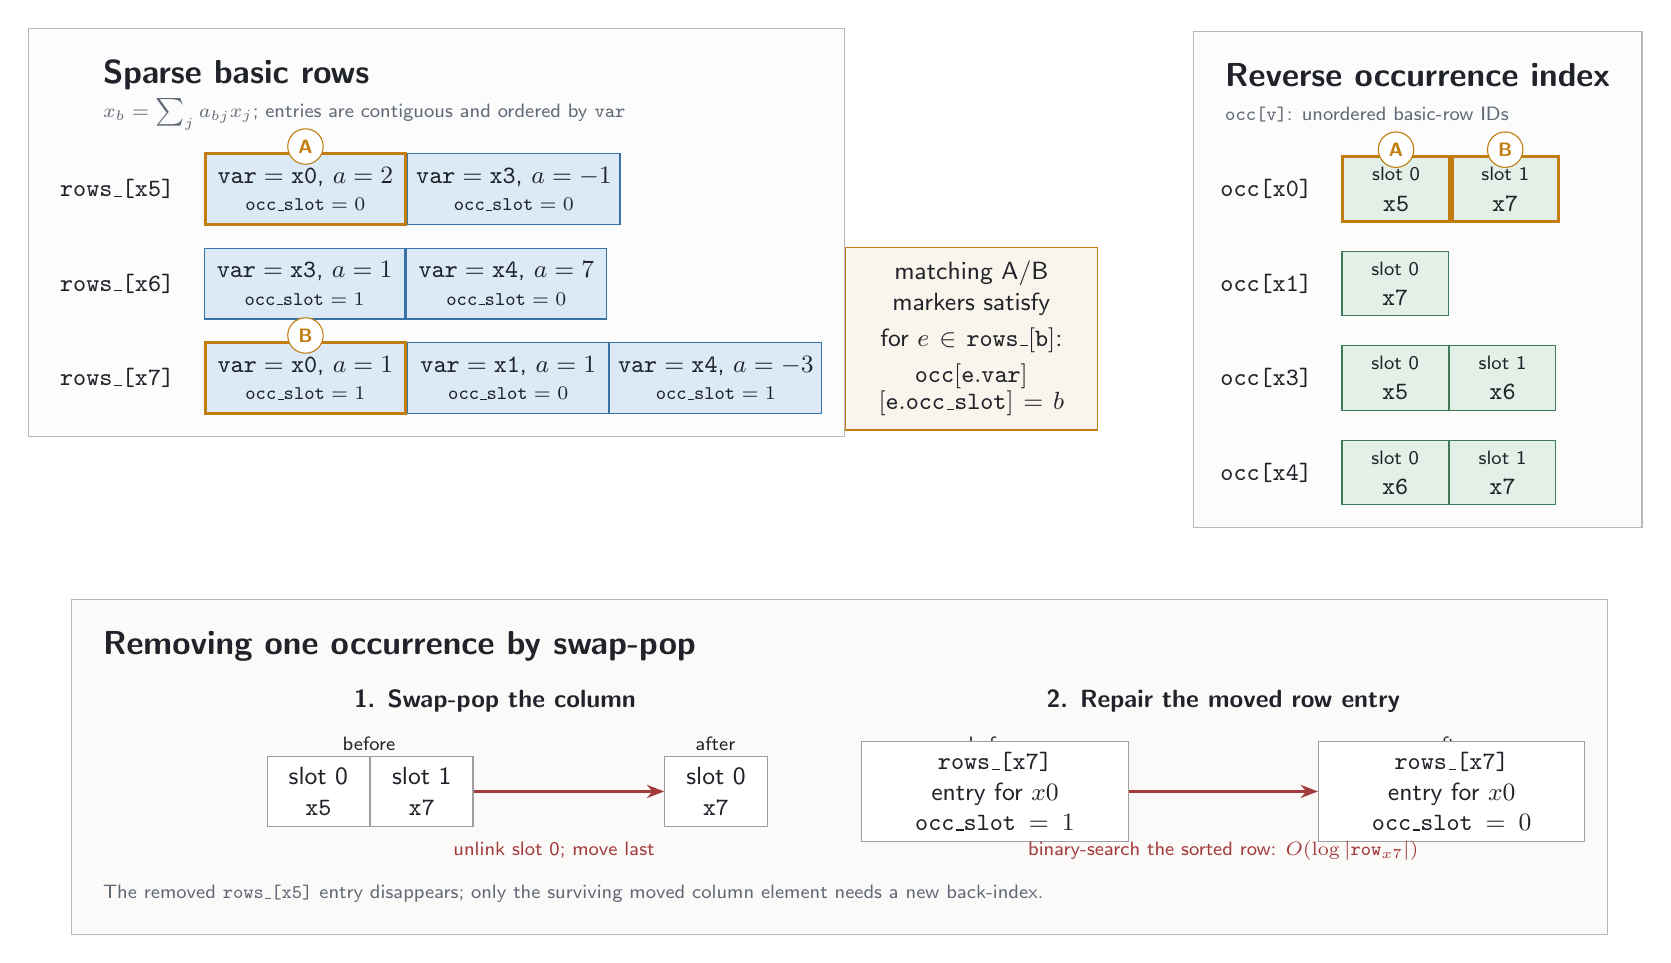
\begin{tikzpicture}[
  font=\sffamily,
  text=ink,
  row entry/.style={
    draw=rowblueborder,
    fill=rowblue,
    minimum width=2.55cm,
    minimum height=0.90cm,
    align=center,
    inner sep=3pt,
    font=\sffamily\small
  },
  column slot/.style={
    draw=colgreenborder,
    fill=colgreen,
    minimum width=1.35cm,
    minimum height=0.82cm,
    align=center,
    inner sep=3pt,
    font=\sffamily\small
  },
  linked entry/.style={draw=accentgold, line width=1.05pt},
  link marker/.style={
    circle,
    draw=accentgold,
    fill=white,
    text=accentgold,
    minimum size=4.5mm,
    inner sep=0pt,
    font=\sffamily\bfseries\scriptsize
  },
  array label/.style={font=\sffamily\bfseries\small, anchor=east},
  panel/.style={draw=black!28, fill=black!1, inner sep=8pt},
  operation arrow/.style={-{Stealth[length=2.2mm]}, draw=repairred, line width=1pt},
  operation box/.style={
    draw=black!38,
    fill=white,
    minimum height=0.78cm,
    align=center,
    inner sep=4pt,
    font=\sffamily\small
  }
]

% Sparse rows: each vector stores only its nonzero entries, ordered by var.
\node[font=\sffamily\bfseries\large, anchor=west] (rows title) at (0,3.80)
  {Sparse basic rows};
\node[font=\sffamily\scriptsize, text=muted, anchor=west] at (0,3.30)
  {$x_b = \sum_j a_{bj}x_j$; entries are contiguous and ordered by \texttt{var}};

\node[array label] (r5 label) at (1.15,2.35) {\texttt{rows\_[x5]}};
\node[row entry, linked entry, anchor=west] (r5x0) at (1.40,2.35)
  {$\mathtt{var=x0}$, $a=2$\\[-1pt]\scriptsize $\mathtt{occ\_slot}=0$};
\node[row entry, right=0pt of r5x0] (r5x3)
  {$\mathtt{var=x3}$, $a=-1$\\[-1pt]\scriptsize $\mathtt{occ\_slot}=0$};

\node[array label] (r6 label) at (1.15,1.15) {\texttt{rows\_[x6]}};
\node[row entry, anchor=west] (r6x3) at (1.40,1.15)
  {$\mathtt{var=x3}$, $a=1$\\[-1pt]\scriptsize $\mathtt{occ\_slot}=1$};
\node[row entry, right=0pt of r6x3] (r6x4)
  {$\mathtt{var=x4}$, $a=7$\\[-1pt]\scriptsize $\mathtt{occ\_slot}=0$};

\node[array label] (r7 label) at (1.15,-0.05) {\texttt{rows\_[x7]}};
\node[row entry, linked entry, anchor=west] (r7x0) at (1.40,-0.05)
  {$\mathtt{var=x0}$, $a=1$\\[-1pt]\scriptsize $\mathtt{occ\_slot}=1$};
\node[row entry, right=0pt of r7x0] (r7x1)
  {$\mathtt{var=x1}$, $a=1$\\[-1pt]\scriptsize $\mathtt{occ\_slot}=0$};
\node[row entry, right=0pt of r7x1] (r7x4)
  {$\mathtt{var=x4}$, $a=-3$\\[-1pt]\scriptsize $\mathtt{occ\_slot}=1$};

% Reverse occurrence index: columns contain basic-row IDs and are unordered.
\node[font=\sffamily\bfseries\large, anchor=west] (occ title) at (14.25,3.80)
  {Reverse occurrence index};
\node[font=\sffamily\scriptsize, text=muted, anchor=west] (occ subtitle) at (14.25,3.30)
  {\texttt{occ[v]}: unordered basic-row IDs};

\node[array label] at (15.60,2.35) {\texttt{occ[x0]}};
\node[column slot, linked entry, anchor=west] (o0s0) at (15.85,2.35)
  {\scriptsize slot 0\\$\mathtt{x5}$};
\node[column slot, linked entry, right=0pt of o0s0] (o0s1)
  {\scriptsize slot 1\\$\mathtt{x7}$};

\node[array label] at (15.60,1.15) {\texttt{occ[x1]}};
\node[column slot, anchor=west] (o1s0) at (15.85,1.15)
  {\scriptsize slot 0\\$\mathtt{x7}$};

\node[array label] at (15.60,-0.05) {\texttt{occ[x3]}};
\node[column slot, anchor=west] (o3s0) at (15.85,-0.05)
  {\scriptsize slot 0\\$\mathtt{x5}$};
\node[column slot, right=0pt of o3s0] (o3s1)
  {\scriptsize slot 1\\$\mathtt{x6}$};

\node[array label] at (15.60,-1.25) {\texttt{occ[x4]}};
\node[column slot, anchor=west] (o4s0) at (15.85,-1.25)
  {\scriptsize slot 0\\$\mathtt{x6}$};
\node[column slot, right=0pt of o4s0] (o4s1)
  {\scriptsize slot 1\\$\mathtt{x7}$};

% Matching markers expose the two x0 links without routing across either panel.
\node[link marker, anchor=south] at ([yshift=-1.6mm]r5x0.north) {A};
\node[link marker, anchor=south] at ([yshift=-1.6mm]o0s0.north) {A};
\node[link marker, anchor=south] at ([yshift=-1.6mm]r7x0.north) {B};
\node[link marker, anchor=south] at ([yshift=-1.6mm]o0s1.north) {B};

\node[draw=accentgold, fill=accentgold!8, align=center, inner sep=5pt,
  text width=2.85cm, font=\sffamily\small] (invariant) at (11.15,0.45)
  {matching A/B markers satisfy\\[2pt]
   for $e \in \mathtt{rows\_[b]}$:\\[2pt]
   $\mathtt{occ[e.var]}$\\[-1pt]
   $\mathtt{[e.occ\_slot]}=b$};

% Swap-pop inset: removing slot 0 moves x7 and repairs its surviving row entry.
\node[font=\sffamily\bfseries\large, anchor=west] (repair title) at (0,-3.45)
  {Removing one occurrence by swap-pop};

\node[font=\sffamily\bfseries\small] at (5.10,-4.15) {1. Swap-pop the column};
\node[font=\sffamily\scriptsize] at (3.50,-4.70) {before};
\node[operation box, anchor=west, minimum width=1.30cm] (before0) at (2.20,-5.30)
  {slot 0\\$\mathtt{x5}$};
\node[operation box, right=0pt of before0, minimum width=1.30cm] (before1)
  {slot 1\\$\mathtt{x7}$};

\node[font=\sffamily\scriptsize] at (7.90,-4.70) {after};
\node[operation box, anchor=west, minimum width=1.30cm] (after0) at (7.25,-5.30)
  {slot 0\\$\mathtt{x7}$};
\draw[operation arrow] (before1.east) -- (after0.west);
\node[font=\sffamily\scriptsize, text=repairred] at (5.85,-6.05)
  {unlink slot 0; move last};

\node[font=\sffamily\bfseries\small] at (14.35,-4.15) {2. Repair the moved row entry};
\node[font=\sffamily\scriptsize] at (11.45,-4.70) {before};
\node[operation box, text width=3.10cm] (repair before) at (11.45,-5.30)
  {\texttt{rows\_[x7]} entry for $x0$\\$\mathtt{occ\_slot}=1$};
\node[font=\sffamily\scriptsize] at (17.25,-4.70) {after};
\node[operation box, text width=3.10cm] (repair after) at (17.25,-5.30)
  {\texttt{rows\_[x7]} entry for $x0$\\$\mathtt{occ\_slot}=0$};
\draw[operation arrow] (repair before.east) -- (repair after.west);
\node[font=\sffamily\scriptsize, text=repairred] at (14.35,-6.05)
  {binary-search the sorted row: $O(\log |\mathtt{row}_{x7}|)$};

\node[font=\sffamily\scriptsize, text=muted, anchor=west] (repair note) at (0,-6.60)
  {The removed \texttt{rows\_[x5]} entry disappears; only the surviving moved
   column element needs a new back-index.};

\begin{scope}[on background layer]
  \node[panel, fit=(rows title)(r5 label)(r7x4)(r7 label)] {};
  \node[panel, fit=(occ title)(occ subtitle)(o0s0)(o0s1)(o4s0)(o4s1)] {};
  \node[panel, fill=repairred!3,
    fit=(repair title)(before0)(before1)(after0)(repair before)(repair after)(repair note)] {};
\end{scope}

\end{tikzpicture}
\end{document}
